\documentclass[12pt, addpoints]{exam/exam}

\usepackage{hyperref}
%\usepackage{mdframed}
\usepackage{graphicx, caption}	
%\usepackage{array, multicol, tabu}
\usepackage{amsmath, amsthm, amssymb}
\usepackage{comment}
\usepackage{enumitem}
\usepackage{url}
\usepackage{textcomp}
\newcommand{\1}{^{-1}}
\newcommand{\vect}[1]{\mathbf{#1}}
\newcommand{\R}{\mathbb R}
\newcommand{\vstr}{\vspace{\stretch{1}}}
\everymath{\displaystyle}
\setlength{\parindent}{0pt}

\theoremstyle{plain}
\newtheorem{thm}{Theorem}
\newtheorem*{thm*}{Theorem}

%\printanswers
\pointformat{\bf(\thepoints)}
\pointpoints{pt}{pts}
\bonuspointformat{\bf(\thepoints)}
\bonuspointpoints{pt}{pts}

\coverfirstpageheader{\bf MATH 235 (Calculus I) \\
		Fall 2017 \\
		}
		{}
		{{Name:} \underline{\hspace{40ex}} \\
		\vspace{0.5pc}
		Tues 26 Sep 2017}
\coverextraheadheight[2pc]{0in}
\coverfirstpagefooter{}{}{\Large Good luck!}
\coverrunningheader{}
	{Exam 1: Functions and limits}
	{}
\coverrunningheadrule	
\coverrunningfootrule
\coverrunningfooter{Wheeler}{Calc I Fall 2017}{p. \thepage\ (of \numpages)}

\firstpageheader{}
	{Exam 1: Functions and limits}
	{}
\firstpageheadrule
\firstpagefootrule
\firstpagefooter{Wheeler}{Calc I Fall 2017}{p. \thepage\ (of \numpages)}

\runningheadrule
\runningheader{}
	{Exam 1: Functions and limits}
	{}
\runningfootrule
\runningfooter{Wheeler}{Calc I Fall 2017}{p. \thepage\ (of \numpages)}

\title{\vspace{-8pc}
\vfill{\Huge
	\bf Exam 1: Functions and limits, v.B \\ (\S1.1-1.5, 2.2-2.6)} 
	}
%\author{}
\date{}

% % % % % % % % % % % % % % % % % % % %
\begin{document}

\begin{coverpages}
\maketitle
\thispagestyle{headandfoot}
\vspace{-4pc}
{\bf Exam Instructions:} You have 75 minutes to complete this exam.  Justification is required for all problems.  Notation matters!  You will also be penalized for missing units and rounding errors.  
No electronic devices (phones, iDevices, computers, etc).  % except for a \textbf{basic scientific calculator}.  On story problems, round to one decimal place. 
If you finish early then you may leave, UNLESS there are less than 5 minutes of class left.  To prevent disruption, if you finish with less than 5 minutes of class remaining then please stay seated and quiet.

\begin{flushright}
%In addition, please provide the following data:

\vspace{0.3in}
%Drill Instructor: \underline{\hspace{40ex}}

\vspace{0.3in}
%Drill Time: \underline{\hspace{40ex}}
\end{flushright}

\vfill
\textbf{Your signature below indicates that you have read this page and agree to follow the Academic Honesty Policies of James Madison University.}  

\vspace{0.3in}
Signature: {\bf (1 pt)} \underline{\hspace{73ex}}

% % % % % % % % % %
\newpage
\vspace*{\fill}
\gradetable
%\textbf{Formulas you may need:}
%\vspace{-2pc}
%\begin{center}
%\vspace*{\fill}
%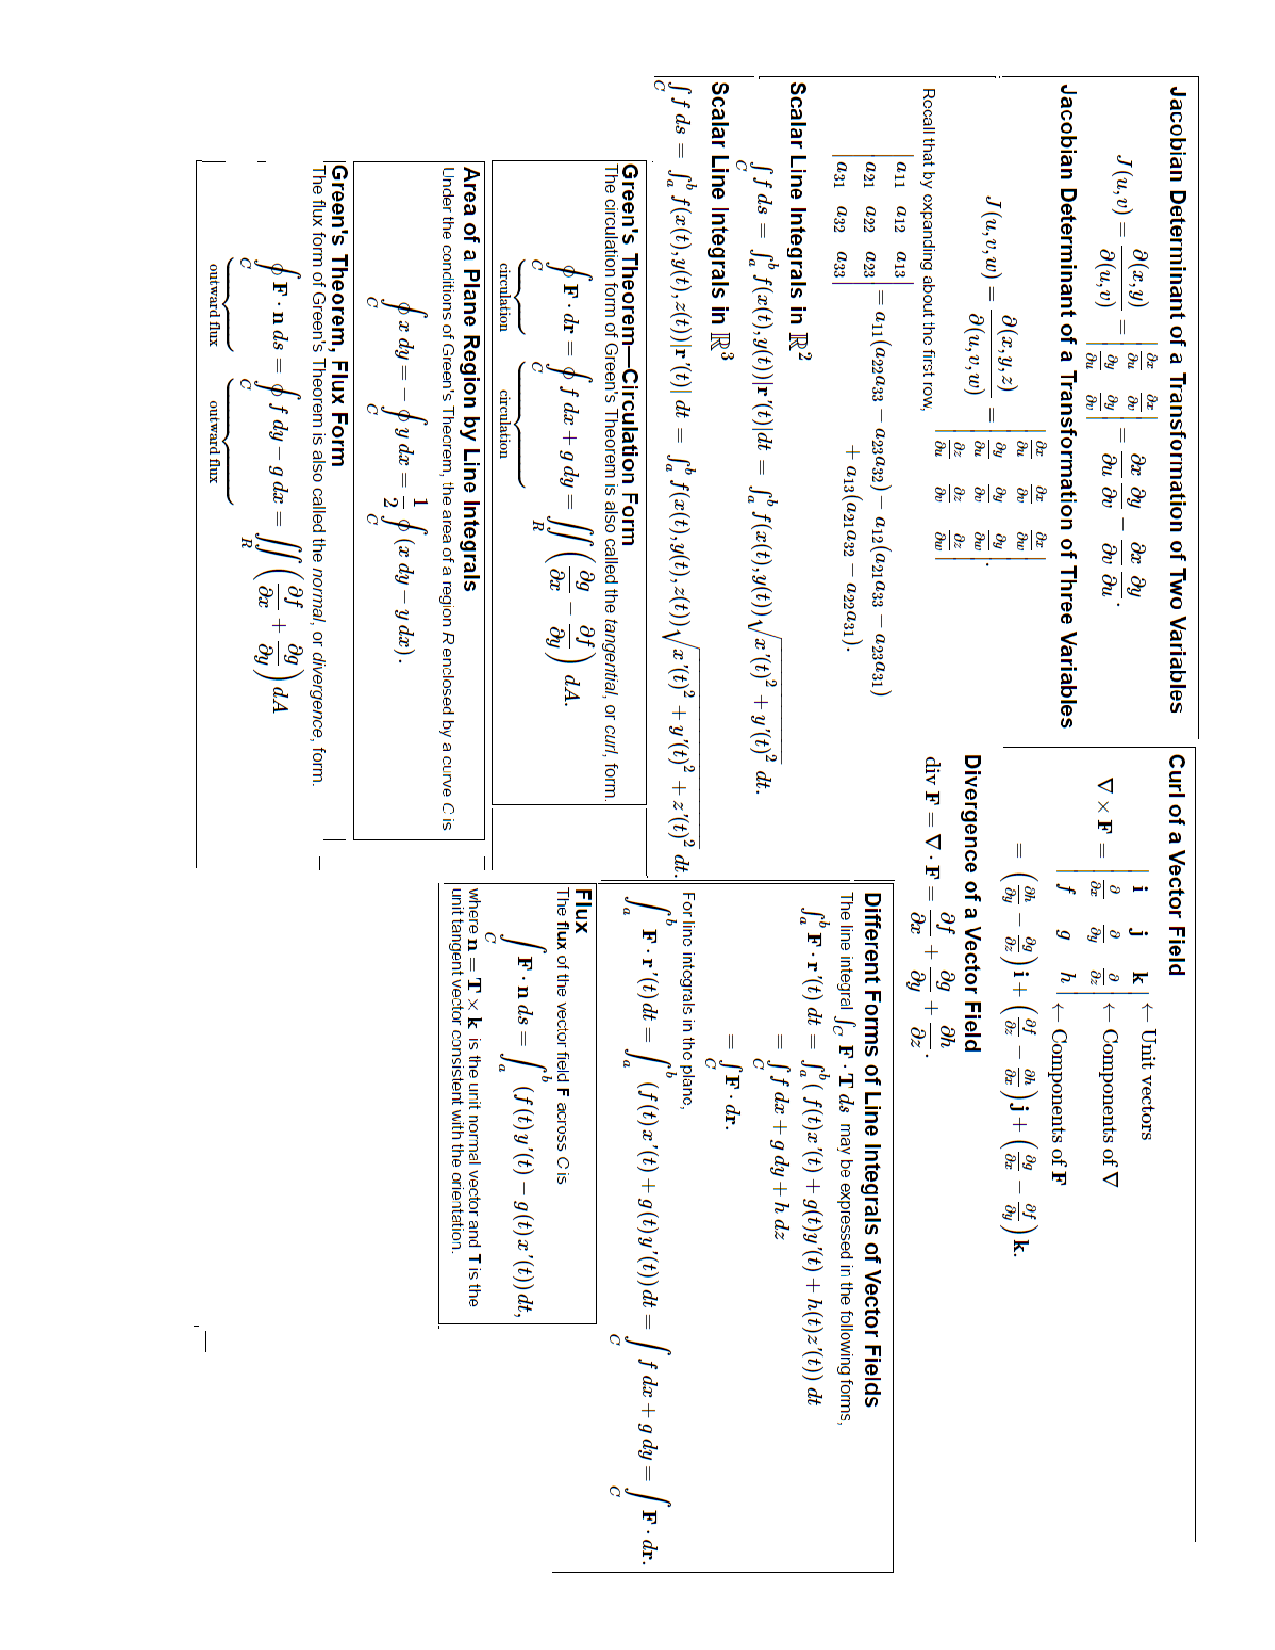
\includegraphics[scale=0.84]{Exam3FormulaSheet.pdf}
%\vspace*{\fill}
%\end{center}
\end{coverpages}

% % % % % % % % % % % % % % % % % % % %
\begin{questions}
\thispagestyle{headandfoot}

\newpage
% % % % %
\question[18] %{\bf \S2.2 \#18} 
Sketch the graph of an example of a function $f$ that satisfies all of the given conditions.
	\begin{itemize}
	\item $\lim_{x\to 0^+}f(x)=0$
	\item $\lim_{x\to 1}f(x)=\infty$		
	\item $f(0)=3$
	\item $\lim_{x\to 0^-}f(x)=3$
	\item $\lim_{x\to -\infty}f(x)=1$
	\item $\lim_{x\to \infty}f(x)=0$
	\item $\lim_{x\to 3^-}f(x)=3$
	\item $f(3)=1$
	\item $\lim_{x\to 3^+}f(x)=0$	
	\end{itemize}

\vfill	
% % % % %
\question%[] {\bf 1.3 \#56} 
A spherical balloon is being inflated and the radius of the balloon is increasing at a rate of 3 cm/s.
	\begin{parts}
	\part[4] Express the radius $r$ of the balloon as a function of the time $t$ (in seconds).
	\vspace{5pc}
	
	\part[6] If $V=\frac{4}{3}\pi r^3$ is the volume of the balloon as a function of the radius, find $V\circ r$ and interpret it.
	\vspace{8pc}
	\end{parts}	
\vfill	

\newpage
% % % % %
\question[15] %{\bf \S2.4 \#18} 
The formal definition of a limit says: $\lim_{x\to a}f(x)=L$ means for every $\epsilon>0$, there exists $\delta>0$, such that $\text{if }0<|x-a|<\delta \text{ then }|f(x)-L|<\epsilon$.

\vspace{1.5pc}
Prove, using the formal definition of a limit, that
\[
\lim_{x\to -1}(2x+1)=-1.
\]

\newpage
% % % % %
\question[20] %{\bf \S2.5 \#46} 
Using the continuity checklist, find the values of $a$ and $b$ that make $f$ continuous at $2$ and $3$.
\[
f(x)=\begin{cases}
	\frac{x^2-4}{x-2} & \text{ if }x<2 \\
	ax^2-bx+3 & \text{ if }2\leq x<3 \\
	2x-a+b & \text{ if }x\geq 3
	\end{cases}
\]

\newpage	
% % % % %
\question %{\bf \S2.3 \#6, 16, 30} 
Evaluate the limits.  You must show work.
\vspace{1pc}  
	\begin{parts}
	%\part $\lim_{x\to -1}\frac{2x^2+3x+1}{x^2-2x-3}$
	\part[4] $\lim_{u\to -4}\frac{\sqrt{u^2+9}-5}{u+4}$
	\vspace{9pc}	
	\part[4] $\lim_{u\to -2}\sqrt{u^4+3u+6}$
	\vspace{9pc}
	\part[4] $\lim_{x\to -\infty}\frac{\sqrt{3x^2+1}}{2x-5}$
	\vspace{9pc}
	%\part $\lim_{x\to -\infty}\frac{4x^3+6x^2-2}{2x^3-4x+5}$
	%\part $\lim_{x\to \infty}(e^{-x}+2\cos{3x})$
	%\part $\lim_{x\to \infty}\frac{e^{3x}-e^{-3x}}{e^{3x}+e^{-3x}}$
	%\part $\lim_{x\to \infty}\frac{\sin^2x}{x^2+1}$
	\part[4] $\lim_{x\to \infty}\frac{1-x^2}{x^3-x+1}$
	\vspace{9pc}
	\end{parts}

\newpage
% % % % %
\question%[] {\bf \S1.4 \#18} 
	\begin{parts}
	\part[5] Sketch, on the same axes, the graph $y=e^x$ and its reflection about the line $y=5$.
	\vspace{12pc}
	
	\part[7] Find the equation of the graph that results from reflecting $y=e^x$ about the line $y=5$.
	\vspace{5pc}
	%\part[] reflecting about the line $x=2$.
	\end{parts}
\vfill

% % % % %
\question%[] %{\bf 1.5 36, 38, 40} 
Simplify each expression.
\vspace{1pc}
	\begin{parts}
	%\part[] $\log_5{1/125}$
	\part[2] $e^{\ln{\ln{e^x}}}$
	\vspace{3pc}	
	\part[2] $\ln(1/e^y)$
	\vspace{3pc}
	\part[2] $3\ln A+2\ln B-\ln C$
	\vspace{3pc}
	\part[2] $e^{-\ln z}$
	\vspace{3pc}
	\end{parts}

\vfill

% % % % %
%\question[] {\bf \S1.4 \#20} Find the domain of each function.
%	\begin{parts}
%	\part[] $g(t)=\sqrt{10^t-100}$
%	\part[] $g(t)=\sin(e^t-1)$
%	\end{parts}	

% % % % %
%\question[] {\bf \S1.4 \#30}
%A bacteria culture starts with 500 bacteria and deoubles in size every half hour.
%	\begin{parts}
%	\part[] How many bacteria are there after 3 hours?
%	\part[] How many bacteria are there after $t$ hours?
%	\part[] How many bacteria are there after 40 minutes?
%	\part[] Graph the population function and estimate the time for the population to reach 100,000.
%	\end{parts}
	
%\newpage

% % % % % 
%\question[] {\bf \S1.4 \#22} Find the exponential function $f(x)=Cb^x$ whose graph is given.
%
%\vspace{-1pc}
%\begin{center}
%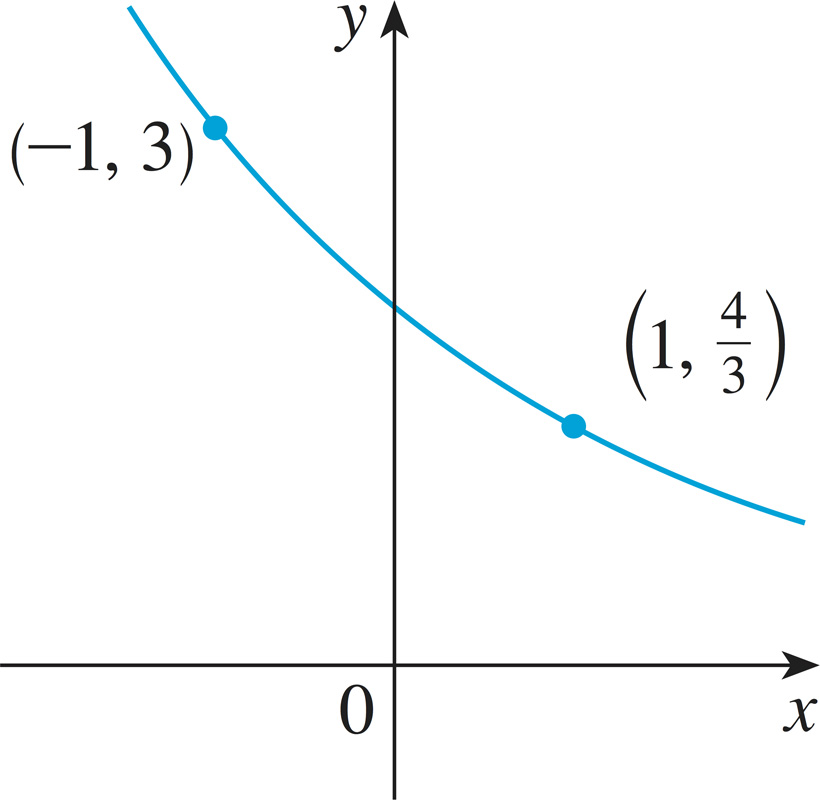
\includegraphics[scale=5]{1-4_22Stewart8Ed}
%\end{center}

% % % % %
%\question[] {\bf 1.5 \#22} Find a formula for the inverse of the function.
%\[
%f(x)=\frac{4x-1}{2x+3}
%\]	

%\newpage
% % % % %
%\question[] {\S1.5 \#62} When a camera flash goes off, the batteries immediately begin to recharge the flash's capacitor, which stores electric charge given by 
%\[
%Q(t)=Q_0(1-e^{-t/a})
%\]
%(The maximum charge capacity is $Q_0$ and $t$ is measured in seconds.)
%	\begin{parts}
%	\part[] Find the inverse of this function and explain its meaning.
%	\part[] How long does it take to rechare the capacitor to 90\% of capacity if $a=2$?
%	\end{parts}

% % % % %
%\question[] Use the given graph of $f$ to sketch the graph of $f\1$.
%\vspace{-1pc}
%\begin{center}
%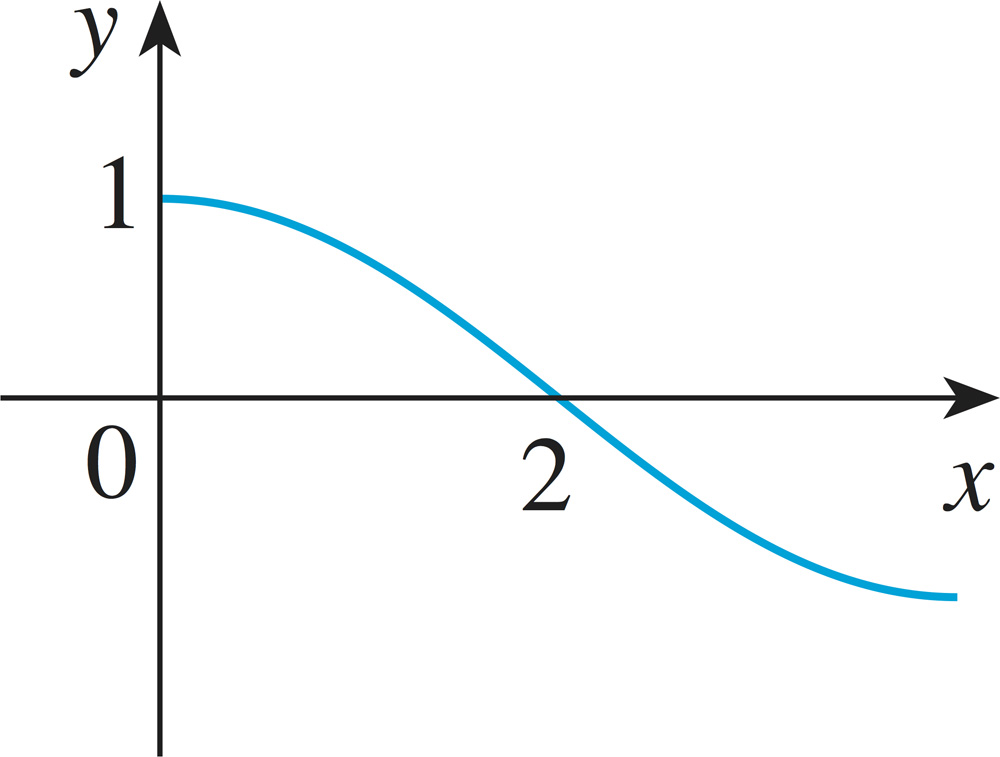
\includegraphics[scale=5]{1-5_30Stewart8Ed}
%\end{center}

% % % % %
%\question[] {\bf 1.5 48, 50} For each of the following, find the domain and range.  Find the $x$-intercept of the graph.  Sketch the graph.
%	\begin{parts}
%	\part[] $y=\ln(-x)$
%	\part[] $y=\ln|x|$
%	\part[] $f(x)=\ln(x-1)-1$
%	\end{parts}

% % % % %
%\question[] The graph of $f$ is given.
%\vspace{-1pc}
%\begin{center}
%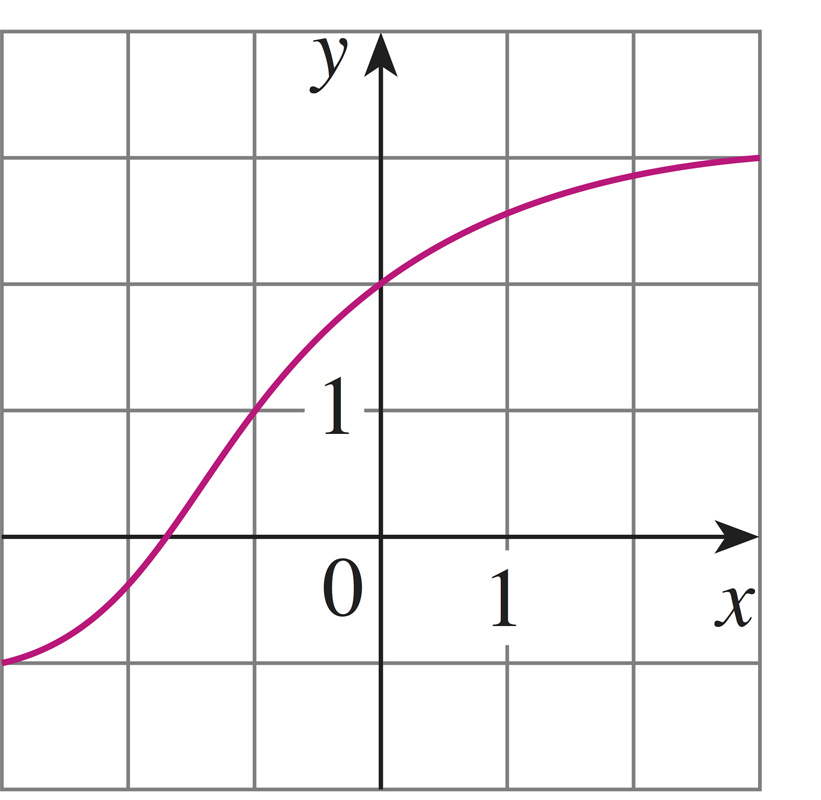
\includegraphics[scale=5]{1-5_18Stewart8Ed}
%\end{center}
%	\begin{parts}
%	\part[] Why is $f$ one-to-one?
%	\part[] What are the domain and range of $f\1$?
%	\part[] What is the value of $f\1(2)$?
%	\part[] Estimate the falue of $f\1(0)$.
%	\end{parts}

% % % % %
%\question[] {\bf 2.2 8} For the function $A$ whose graph is shown, state the following:
%	\begin{parts}
%	\part[] $\lim_{x\to -3}A(x)$
%	\part[] $\lim_{x\to 2^-}A(x)$
%	\part[] $\lim_{x\to 2^+}A(x)$
%	\part[] $\lim_{x\to -1}A(x)$
%	\part[] the equations of the vertical asymptotes.
%	\end{parts}
%\vspace{-1pc}
%\begin{center}
%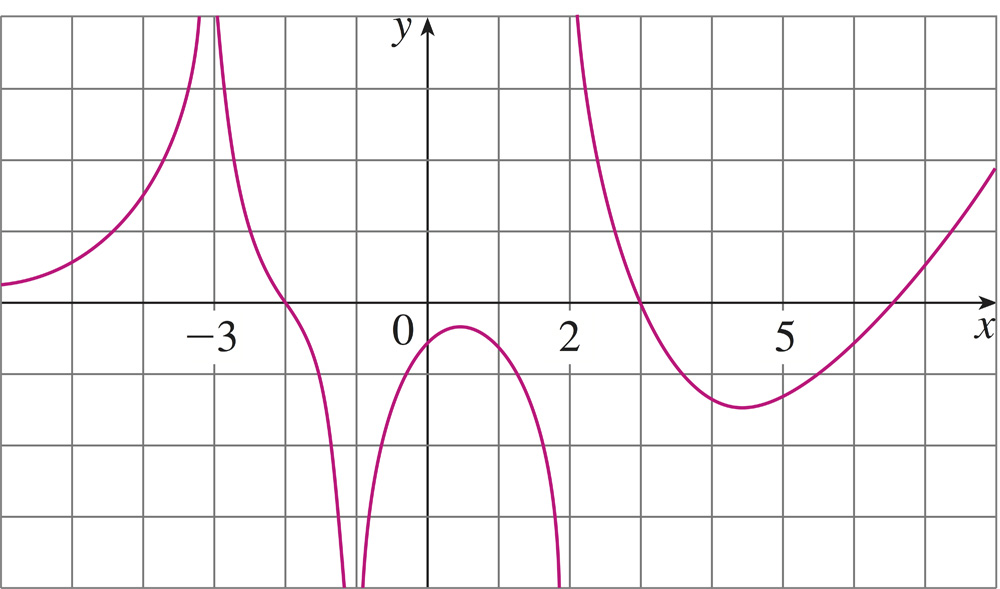
\includegraphics[scale=5]{2-2_8Stewart8Ed}
%\end{center}	
	
% % % % %
%\question[] {\bf \S2.3 \#2} The graphs of $f$ and $g$ are given.  Use them to evaluate each limit, if it exists.  If the limit does not exist, explain why.
%	\begin{parts}
%	\part $\lim_{x\to 2}(f(x)+g(x))$
%	\part $\lim_{x\to -1}f(x)g(x)$
%	\part $\lim_{x\to 2}x^2f(x)$
%	\part $\lim_{x\to 0}(f(x)-g(x))$
%	\part $\lim_{x\to 3}\frac{f(x)}{g(x)}$
%	\part $f(-1)+\lim_{x\to -1}g(x)$
%	\end{parts}
%
%{\bf NEED THE GRAPHS}
	
% % % % %
%\question[] {\bf \S2.3 \#38} Given $2x\leq g(x)\leq x^4-x^2+2$ for all $x$, evaluate $\lim_{x\to 1}g(x)$. 
	
% % % % %
%\question[] {\bf \S2.4 \#42} Prove, using Definition 6, that $\lim_{x\to -3}\frac{1}{(x+3)^4}=\infty$.	

% % % % %
%\question[] {\bf \S1.4 \#2,4}  Rewrite and simplify the following expressions:
%	\begin{parts}
%	\part[] $8^{4/3}$
%	\part[] $x(3x^2)^3$
%	\part[] $\frac{x^{2n}\cdot x^{3n-1}}{x^{n+2}}$
%	\part[] $\frac{\sqrt{a\sqrt b}}{\sqrt[3]{ab}}$
%	\end{parts}

% % % % % 
%\question[] {\bf \S2.6 \#16, 18, 32, 36, 38} Compute each limit or explain why it doesn't exist.
%	\begin{parts}
%	\part $\lim_{x\to \infty}\frac{1-x^2}{x^3-x+1}$
%	\part $\lim_{x\to -\infty}\frac{4x^3+6x^2-2}{2x^3-4x+5}$
%	\part $\lim_{x\to \infty}(e^{-x}+2\cos{3x})$
%	\part $\lim_{x\to \infty}\frac{e^{3x}-e^{-3x}}{e^{3x}+e^{-3x}}$
%	\part $\lim_{x\to \infty}\frac{\sin^2x}{x^2+1}$
%	\part $\lim_{x\to -\infty}\frac{\sqrt{2x^2+1}}{3x-5}$
%	\end{parts}


% % % % %
%\question[] {\bf \S1.1 \#14} Three runners compete in a 100 m race.  The graph depicts the distance run as a function of time for each runner.  Who won?  Who finished the race?  Who started out ahead?
%
%\vspace{-1pc}
%\begin{center}
%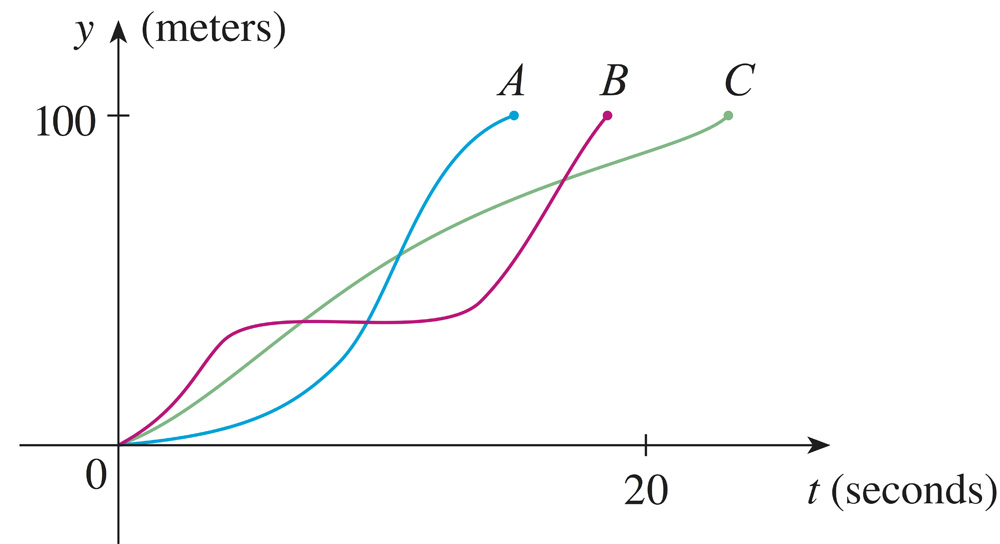
\includegraphics[scale=7]{1-1_14Stewart8Ed}
%\end{center}

% % % % %
%\question[] {\bf \S1.3 \#52} Use the table to evaluate each expression.
%	\begin{parts}
%	\part $f(g(1))$
%	\part $g(g(1))$
%	\part $g(f(1))$
%	\part $(g\circ f)(3)$
%	\part $(f\circ g)(6)$
%	\end{parts}
%	
%{\bf PUT THE TABLE HERE}	

\end{questions}

\end{document}